
\begin{frame}<0>[fragile,label=storedXSS]{stored cross-site scripting}
\begin{tikzpicture}
    \node[draw,thick,inner sep=5mm,align=left,text=red!70!black,align=left] (commentBox) {
\begin{lstlisting}[language={}]
<script>
    document.location = 'http://attacker.com';
</script>
\end{lstlisting}
    };
    \node[anchor=south west] at (commentBox.north west) { Your comment: };
    \node[align=left,anchor=north west] (nameLabel) at (commentBox.south west) {
        Name: 
    };
    \node[draw,font=\tt,thick,inner sep=1mm,align=left,text=red!70!black,anchor=west,minimum width=5cm] at (nameLabel.east) {
        An Attacker
    };
\end{tikzpicture}
\end{frame}

\begin{frame}[fragile,label=storedXSS2]{stored cross-site scripting}
    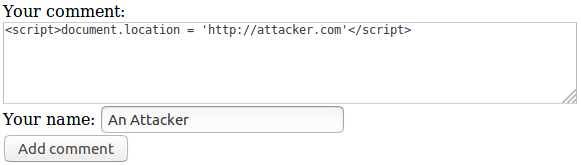
\includegraphics[width=\textwidth]{../web/stores-xss}
\end{frame}

\begin{frame}{scripts on webpages}
    \begin{itemize}
    \item this example: redirect someone reading comment to other website
    \item common proof of concept: make alert box
    \vspace{.5cm}
    \item not especially useful for most attacker goals
    \end{itemize}
\end{frame}
